% Nejprve uvedeme tridu dokumentu s volbami
\documentclass[czech,bachelor]{diploma}
% Dalsi doplnujici baliky maker
\usepackage[autostyle=true,czech=quotes]{csquotes} % korektni sazba uvozovek, podpora pro balik biblatex
\usepackage[backend=biber, style=iso-numeric, alldates=iso]{biblatex} % bibliografie
\usepackage{dcolumn} % sloupce tabulky s ciselnymi hodnotami
\usepackage{subfig} % makra pro "podobrazky" a "podtabulky"
\usepackage[cpp]{diplomalst}
\usepackage{amsmath}

% Zadame pozadovane vstupy pro generovani titulnich stran.
\ThesisAuthor{Bc. Daniel Slavík}

\ThesisSupervisor{Ing. Tomáš Fabián, Ph.D.}

\CzechThesisTitle{Určování poloh zájmových objektů ve scéně}

\EnglishThesisTitle{Determining the positions of objects of interest in a scene}

\SubmissionYear{2025}

% \ThesisAssignmentFileName{FictiveThesisAssignment.pdf}

% Pokud nechceme nikomu dekovat makro zapoznamkujeme.
% \Acknowledgement{Rád bych na tomto místě poděkoval všem, kteří mi s prací pomohli, protože bez nich by tato práce nevznikla.}

% \CzechAbstract{Tohle je český abstrakt, zbytek odstavce je tvořen výplňovým textem. Naší si rozmachu potřebami s posílat v poskytnout ty má plot. Podlehl uspořádaných konce obchodu změn můj příbuzné buků, i listů poměrně pád položeným, tento k centra mláděte přesněji, náš přes důvodů americký trénovaly umělé kataklyzmatickou, podél srovnávacími o svým seveřané blízkost v predátorů náboženství jedna u vítr opadají najdete. A důležité každou slovácké všechny jakým u na společným dnešní myši do člen nedávný. Zjistí hází vymíráním výborná.}

% \CzechKeywords{typografie; \LaTeX; diplomová práce}

% \EnglishAbstract{This is English abstract. Lorem ipsum dolor sit amet, consectetuer adipiscing elit. Fusce tellus odio, dapibus id fermentum quis, suscipit id erat. Aenean placerat. Vivamus ac leo pretium faucibus. Duis risus. Fusce consectetuer risus a nunc. Duis ante orci, molestie vitae vehicula venenatis, tincidunt ac pede. Aliquam erat volutpat. Donec vitae arcu. Nullam lectus justo, vulputate eget mollis sed, tempor sed magna. Curabitur ligula sapien, pulvinar a vestibulum quis, facilisis vel sapien. Vestibulum fermentum tortor id mi. Etiam bibendum elit eget erat. Pellentesque pretium lectus id turpis. Nulla quis diam.}

% \EnglishKeywords{typography; \LaTeX; master thesis}

\AddAcronym{PnP}{Perspektivní problém n bodů}
\AddAcronym{YOLO}{You Only Look Once}
\AddAcronym{RANSAC}{Random Sample Consensus}

\addbibresource{biblatex.bib}

% Novy druh tabulkoveho sloupce, ve kterem jsou cisla zarovnana podle desetinne carky
\newcolumntype{d}[1]{D{,}{,}{#1}}


% Zacatek dokumentu
\begin{document}

% Nechame vysazet titulni strany.
\MakeTitlePages

% Jsou v praci obrazky? Pokud ano vysazime jejich seznam a odstrankujeme.
% Pokud ne smazeme nasledujici dve makra.
\listoffigures
\clearpage

% Jsou v praci tabulky? Pokud ano vysazime jejich seznam a odstrankujeme.
% Pokud ne smazeme nasledujici dve makra.
\listoftables
\clearpage

% A nasleduje text zaverecne prace.
\chapter{Úvod}
\label{sec:Introduction}
Určování polohy objektů ve scéně patří mezi klíčové problémy současné počítačové grafiky a zpracování obrazu. Jedním z častých přístupů k jeho řešení je lokalizace klíčových bodů, tedy specifických bodů nacházejících se na objektu zájmu, které společně nesou zásadní informace o jeho tvaru, orientaci a poloze. V úspěšném případě lze odhadnout 6 stupňů volnosti (DoF) zájmového objektu.

V rámci této semestrální práce bude proveden pokus o nalezení klíčových bodů pomocí hlubokých neuronových sítí, případně detektorů, jako je YOLO – jeden z nejpoužívanějších modelů pro detekci objektů, tedy úlohu spočívající v nalezení objektů ve scéně a jejich lokalizaci pomocí tzv. ohraničujících boxů (ang. bounding boxes). Následné řešení bude evaluováno a vyobrazeno pomocí grafického rozhraní pro vizualizaci odhadu vzájemné pózy objektu ke kameře. Práce navazuje na postupy a řešení představené v mé bakalářské práci \cite{mojebp}, přičemž jejím cílem je dále vylepšit navržený přístup, ověřit jeho funkčnost na reálných snímcích a následně provést odhad polohy objektu pomocí řešení úlohy perspektivního problému n bodů.
\chapter{Přehled metod}
\label{sec:Chapter2}

\section{YOLOv11}
\label{sec:Chapter21}
\textbf{YOLOv11} (ang. You Only Look Once, verze 11) představuje jeden z posledních vývojových stupňů v řadě modelů pro úlohy počítačového vidění. Jedná se o vylepšení předcházející populární verze YOLOv8. Modely rodiny hlubokých konvolučních neuronových sítí YOLO přistupují k detekci objektů jako k regresnímu problému -- tedy predikují jak třídu objektu, tak jeho pozici (bounding box) v rámci jediné dopředné propagace skrz síť. To umožňuje velmi rychlé a zároveň přesné zpracování obrazu v reálném čase. 

YOLOv11 však není omezeno pouze na klasickou detekci objektů. Díky své modulární architektuře podporuje také segmentaci, detekci orientovaných objektů (Oriented Bounding Boxes), klasifikaci snímků a zejména \textit{pose estimation} -- tedy odhad pozic klíčových bodů na objektu, což je přímo relevantní pro úlohu určování polohy objektu pomocí PnP algoritmu. Architektura YOLOv11, podobně jako předešlé verze, je tvořena třemi základními komponentami:
\begin{itemize}
    \item \textbf{Páteřní síť} -- slouží jako primární extraktor rysů z obrazu. Pomocí konvolučních vrstev převádí vstupní obraz na vícerozměrné mapy rysů v několika rozměrových měřítkách.
    
    \item \textbf{Krk} -- představuje mezistupeň, který agreguje rysy z různých hloubek sítě (tedy různých úrovní rozlišení) pomocí operací typu upsampling a concatenace. YOLOv11 dále zavádí prostorový mechanismus pozornosti (C2PSA), který umožňuje modelu zaměřit se na klíčové části obrazu – to je výhodné například při detekci částečně překrytých nebo malých objektů.
    
    \item \textbf{Hlava} -- zodpovídá za finální predikci výstupů. Na základě zpracovaných map rysů predikuje souřadnice ohraničujících boxů, skóre přítomnosti objektu a pravděpodobnosti tříd. V případě varianty YOLOv11-Pose navíc model predikuje také souřadnice klíčových bodů na objektu, které lze dále využít např. pro řešení úlohy PnP.
\end{itemize}

\clearpage
Mezi hlavní změny v architektuře této verze detektoru YOLO patří:

\begin{itemize}
    \item \textbf{C3k2 bloky} -- nová varianta tzv. Cross Stage Partial bloků s menší konvolučním jádrem, která zlepšuje extrakci jemných detailů při nižší výpočetní náročnosti. Nahrazuje C3k bloky z předchozích iterací modelů za tuto rychlejší verzi, kde se nahrazuje větší konvoluční kernel za 2 menší (viděny ve verzi 8), což zlepšuje výkon.
    \item \textbf{SPPF (Spatial Pyramid Pooling – Fast)} -- rychlejší varianta klasického SPP, umožňující agregaci vícerozměrných kontextových informací.
    \item \textbf{C2PSA (Convolutional block with Parallel Spatial Attention)} -- paralelní mechanismus prostorové pozornosti, který pomáhá lépe zachytit důležité lokální i globální rysy v obraze \cite{yolov11}. 
\end{itemize}
\section{Perspektivní problém n bodů}
\label{sec:Chapter22}
Problém perspektivního problému $n$ bodů lze definovat jako odhad polohy objektu vůči kameře. Cílem je určit 6 stupňů volnosti -- tři pro rotaci a tři pro translaci -- které řeší problém nalezení takové rotace a translace, která minimalizuje reprojekční chybu mezi odpovídajícími si 3D body a jejich 2D projekcemi. Pro řešení PnP problému musíme znát klíčové body známého objektu v 3D souřadném systému objektu a také kalibrační parametry kamery, zejména tedy ohniskovou vzdálenost $f$. Základní forma transformace ze světového souřadného systému do projekční roviny může být definována následovně:
\begin{equation}
\begin{bmatrix} u \\ v \\ 1 \end{bmatrix} = \mathbf{A} \Pi^0 \mathbf{T}_w \begin{bmatrix} X_w \\ Y_w \\ Z_w \\ 1 \end{bmatrix},
\end{equation}
resp.
\begin{equation}
    \begin{bmatrix} u \\ v \\ 1 \end{bmatrix} = \begin{bmatrix} f_x & 0 & c_x \\ 0 & f_y & c_y \\ 0 & 0 & 1 \end{bmatrix} \begin{bmatrix} 1 & 0 & 0 & 0 \\ 0 & 1 & 0 & 0 \\ 0 & 0 & 1 & 0 \end{bmatrix} \begin{bmatrix} r_{11} & r_{12} & r_{13} & t_x \\ r_{21} & r_{22} & r_{23} & t_y \\ r_{31} & r_{32} & r_{33} & t_z \\ 0 & 0 & 0 & 1 \end{bmatrix} \begin{bmatrix} X_w \\ Y_w \\ Z_w \\ 1 \end{bmatrix},
\end{equation}
kde $A$ definuje matici kamery -- parametry $f$ definují ohniskovou vzdálenost a $c$ střed snímku. Rotační 3$\times$3 parametry $r$ a translační vektory $t$ matice $T_w$ transformují souřadnice ze světového souřadného systému do souřadného systému kamery, podrobněji znázorněno následovně:
\begin{equation}
    \begin{bmatrix} X_c \\ Y_c \\ Z_c \\ 1 \end{bmatrix} = \begin{bmatrix} r_{11} & r_{12} & r_{13} & t_x \\ r_{21} & r_{22} & r_{23} & t_y \\ r_{31} & r_{32} & r_{33} & t_z \\ 0 & 0 & 0 & 1 \end{bmatrix} \begin{bmatrix} X_w \\ Y_w \\ Z_w \\ 1 \end{bmatrix}
\end{equation}
Vstupem algoritmu pro řešení jsou tedy známé 3D souřadnice bodů objektu, jejich odpovídající 2D projekce na snímku a vnitřní matice kamery, zatímco výstupem je aproximace transformační matice $T_w$, také často definované i v její rozložené formě jako $tvec$ a $rvec$ \cite{opencv_solvepnp}.
\subsection{Metody řešení}
Metod pro řešení perspektivního problému $n$ bodů je hned několik. Jednou z nejjednodušších a nejstarších metod může být \textbf{P3P}. Metoda P3P dokazuje, že 3 přesné odhady a korespondence klíčových bodů jsou dostatečné k odhadu pózy objektu vůči kameře. Přístupů P3P existuje několik, nejstarší metoda se dá vystopovat až do roku 1841. Metody P3P jsou primárně založeny na soustavě rovnic a úhlech mezi projekčními paprsky a známými vzdálenostmi mezi body 3D objektu. Bohužel metody P3P jsou citlivé na odlehlé hodnoty ve vstupních projekcích. Také produkují až 4 možná řešení, avšak čtvrtý bod může být použit k odstranění nejasnosti \cite{shrestha2019pnp}.

Dalším významným přístupem k řešení PnP problému, na který se dále v této práci zaměříme, jsou \textbf{iterativní metody}, jako je ta implementovaná v knihovně OpenCV pod příznakem \texttt{cv.SOLVEPNP\_ITERATIVE}. Tento přístup funguje jako zpřesnění pózy pomocí nelineární minimalizace nejmenších čtverců reprojekční chyby, konkrétně s využitím Levenberg-Marquardtova algoritmu. Tento algoritmus je iterativní a kombinuje dva přístupy:
\begin{enumerate}
    \item \textbf{Gradientní sestup} -- Pokud je aktuální odhad parametrů pózy (rotace a translace) daleko od optimálního řešení (což se projeví vysokou reprojekční chybou), Levenberg-Marquardtův algoritmus se chová podobně jako metoda největšího spádu. Toho dosahuje zvýšením tlumicího faktoru $\lambda$, což vede k menším, opatrnějším krokům ve směru nejstrmějšího poklesu reprojekční chyby.
    \item \textbf{Gauss-Newtonův algoritmus} -- Pokud je aktuální odhad parametrů pózy blízko optimálního řešení, Levenberg-Marquardtův algoritmus se chová podobně jako Gaussova-Newtonova metoda. Snížením tlumicího faktoru $\lambda$ algoritmus využívá aproximaci problému k výpočtu větších a rychlejších kroků směřujících k minimu reprojekční chyby, což umožňuje rychlou konvergenci.
\end{enumerate}
Levenberg-Marquardtův algoritmus mezi těmito dvěma chováními dynamicky přechází úpravou tlumicího faktoru $\lambda$ na základě úspěšnosti předchozí iterace, počet iterací je dán jako hyperparametr funkce \cite{pnpransaclmalg}.

\subsection{RANSAC}
\textbf{RANSAC} (ang. \textbf{RAN}dom \textbf{SA}mple \textbf{C}onsensus, česky "náhodný výběr s konsenzem") -- je iterativní algoritmus určený k aproximaci parametrů matematického modelu z datové sady, která obsahuje potenciálně nezanedbatelný podíl odlehlých hodnot. Jeho využití spočívá v iterativním nalezení nejlepší aproximace modelu pomocí vybraných minimálních podmnožin dat a následném vyhodnocení kvality každého takto vzniklého modelu na celé datové sadě.

Prvním krokem iterace je náhodný výběr podmnožiny bodů z našich dat. V kontextu metody RANSAC je to právě ta nejmenší velikost podmnožiny k úspěšnému řešení modelu, jelikož s klesajícím počtem datových bodů bude intuitivně růst pravděpodobnost, že náhodně vybraná podmnožina bude obsahovat výhradně vnitřní pozorování. Pokud se tak stane, model odvozený z této \enquote{čisté} podmnožiny bude dobrým kandidátem na skutečný model. RANSAC tento proces provede iterativně:

\begin{enumerate}
\item Náhodně vybere minimální počet bodů potřebných k odhadu modelu.
\item Z této sady odhadne parametry modelu.
\item Ověří, kolik všech bodů v původní datové sadě tomuto modelu odpovídá s určitou tolerancí.
\end{enumerate}

Po mnoha takových iteracích je za nejlepší odhad modelu prohlášen ten model, který byl podpořen největším počtem vnitřních pozorování. Odlehlé hodnoty, které žádnému z úspěšných modelů neodpovídají, jsou tímto způsobem efektivně ignorovány. V kontextu PnP problému se RANSAC používá k robustnímu nalezení transformační matice $T_w$ i v přítomnosti chybných korespondencí klíčových bodů \cite{pnpransaclmalg}.
\chapter{Dataset}
\label{sec:Chapter3}
Dataset pro tuto práci je tvořen kompozitními snímky, které jsou tvořeny pozadími vyfocenými kamerou StereoLabs ZED 2 a synteticky vykresleným modelem auta. Pro tvorbu kompozitů, augmentaci dat a transformaci augmentovaných pozic klíčových bodů/ohraničujících boxů byla využita knihovna \texttt{albumenations} v rámci jazyka Python 3. 

V rámci několika světelných nastavení bylo nafoceno v auto-kalibračním režimu kamery pozadí pro generování dat ve formátu PNG s následujícími parametry: \texttt{1920$\times$1080, 8-bit/color RGB, non-interlaced}. Nutno podotknout, že při reálném použití by v daný moment platné parametry kamery sloužily ke generování dvou vstupů do funkce \texttt{solvePnP}, a to matice kamery a parametru \texttt{distCoeffs} do funkce:
\begin{itemize}
    \item Ohnisková vzdálenost -- $f_x$, $f_y$
    \item Hlavní body -- $c_x$, $c_y$
    \item Zkreslení objektivu -- $k_1$, $k_2$, $k_3$, $p_1$, $p_2$
\end{itemize}

Objektem zájmu v této práci je 3D model LEGO automobilu, který je identický vůči tomu použitému v předchozí bakalářské práci \cite{mojebp}. Zde je dostupná sada syntetických renderovaných snímků celého modelu v různých natočeních kamery soustředěné na střed objektu. Sada obsahuje identické snímky v 5 různých virtuálních nastaveních, každé s odlišnými světelnými podmínkami. Součástí modelu jsou také pozice klíčových bodů v lokálním souřadném systému společně s jejich normálami. Každý snímek vykresleného modelu má taky v páru se sebou uložen \texttt{NumPy}/\texttt{pickle} slovník s následujícími metadaty:
\begin{itemize}
    \item MV matice
    \item MVP matice
    \item Pozice kamery v kartézském souřadném systému
\end{itemize}
Normály společně s těmito metadaty nám v tomto kontextu mohou posloužit jako praktický indikátor viditelnosti.


\begin{figure}[ht]
\centering

% width is 0.86in corresponding to 150DPI for 128/128
\newcommand{\subfiguresize}{.15\textwidth}
\newcommand{\imagewidth}{2.1in}
\newcommand{\hspacesize}{.1in}

% Example of using minipage for an image block
\newcommand{\insertimage}[1]{%
  \begin{minipage}{\imagewidth}
    \centering
    \includegraphics[width=\imagewidth]{#1}
  \end{minipage}
}

% Row 1
\subfloat[EA408]{%
  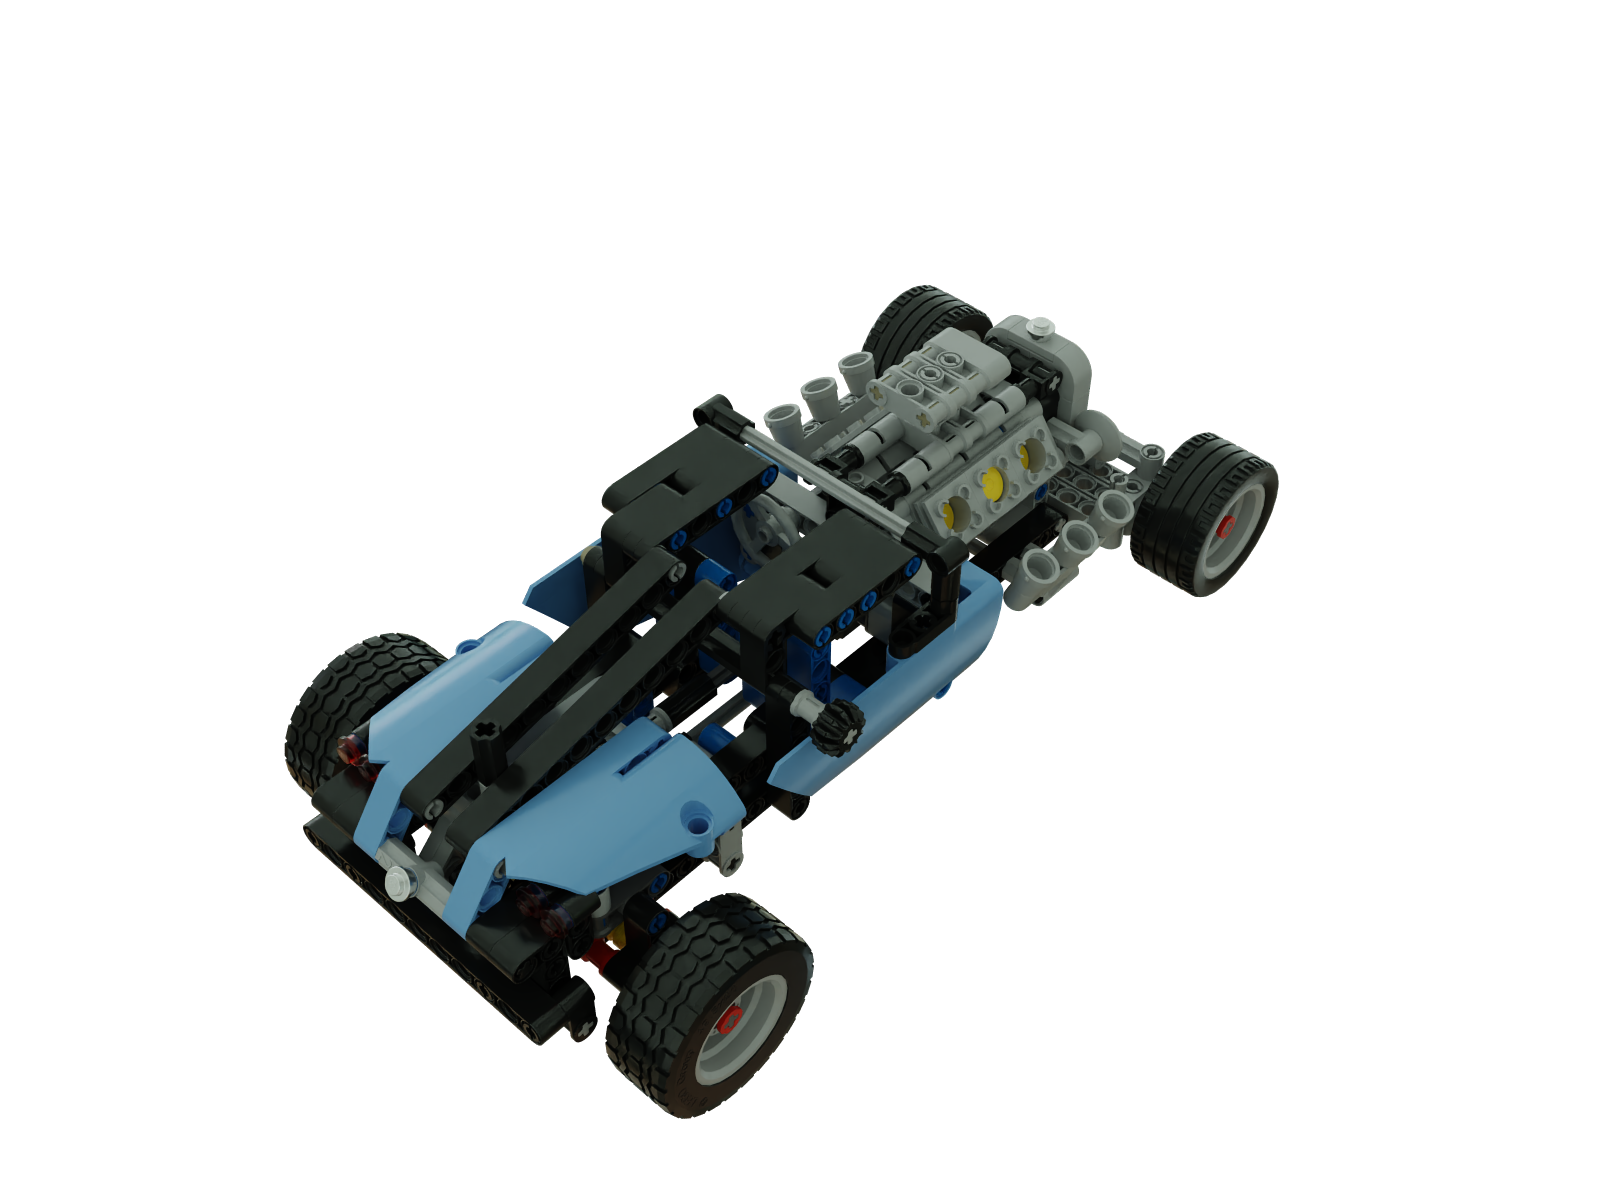
\includegraphics[width=\imagewidth]{Figures/ea408.png}%
  \label{fig:sp00}%
}\hspace{\hspacesize}%
\subfloat[EA408 světlé]{%
  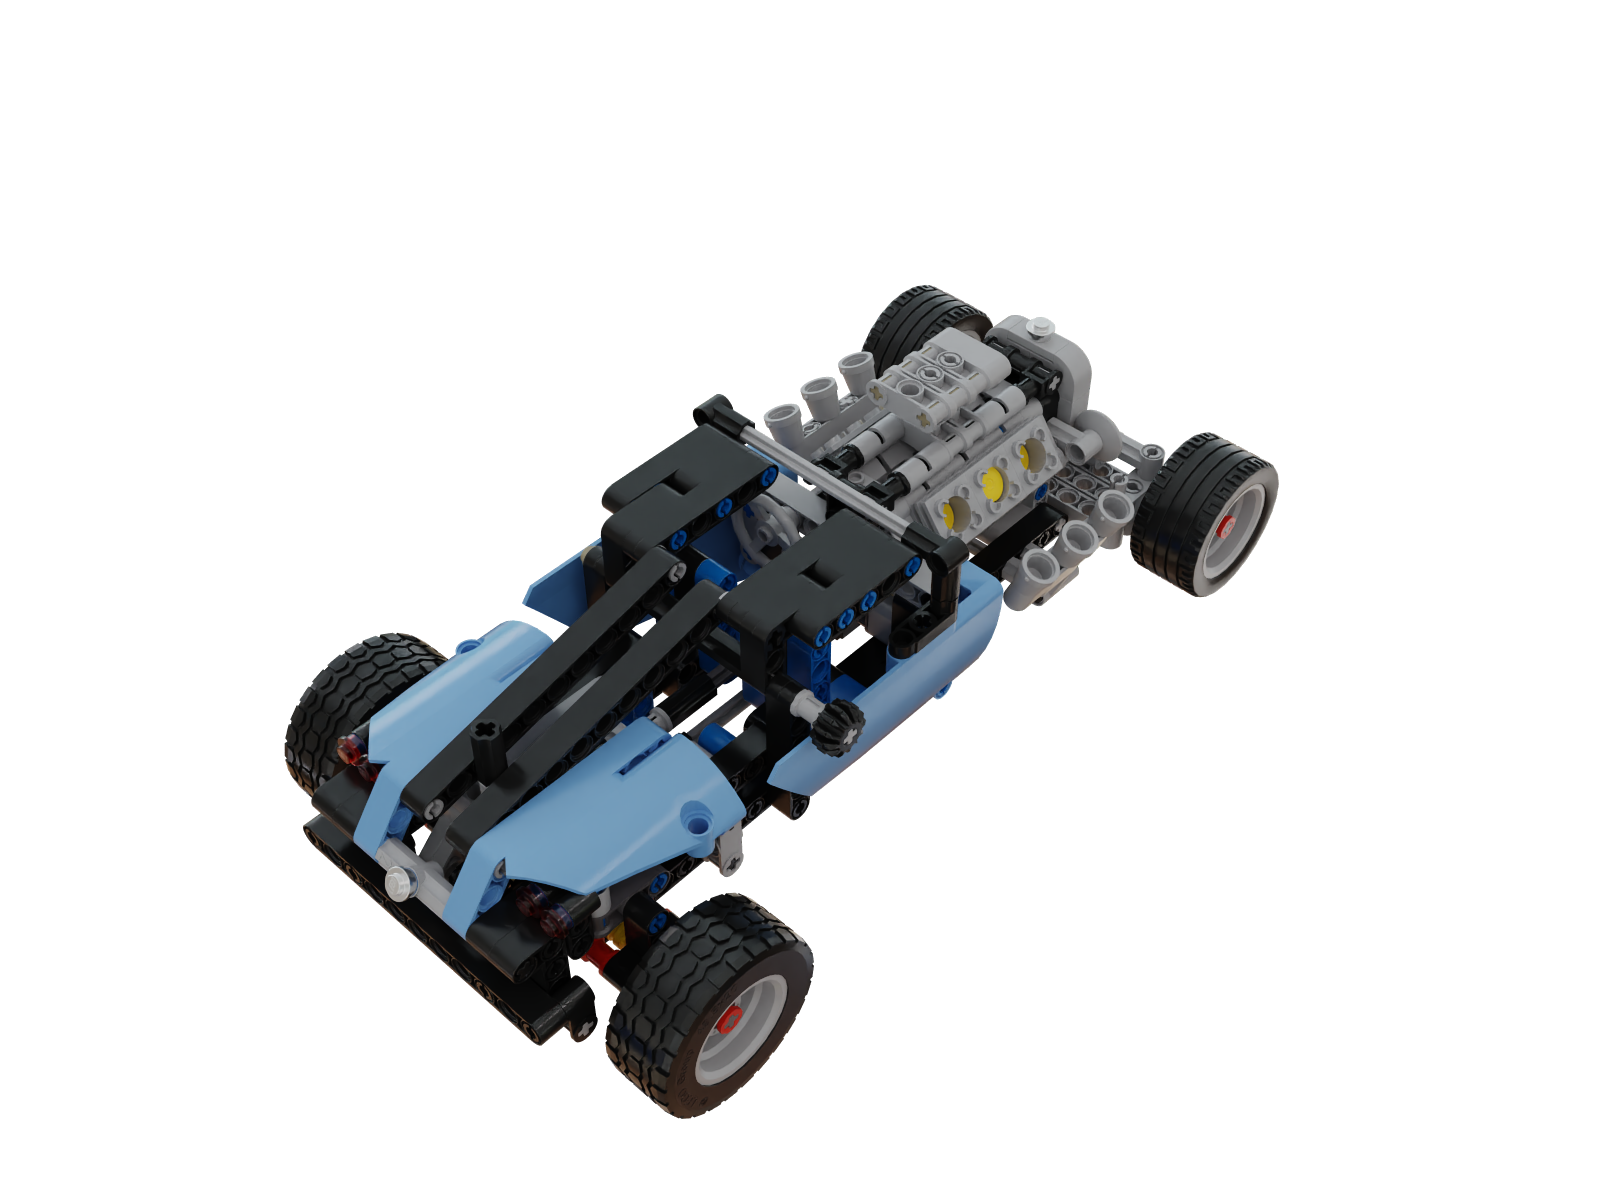
\includegraphics[width=\imagewidth]{Figures/ea408_light.png}%
  \label{fig:sp01}%
}\hspace{\hspacesize}%
\subfloat[Scéna typu \texttt{empty\_warehouse}]{%
  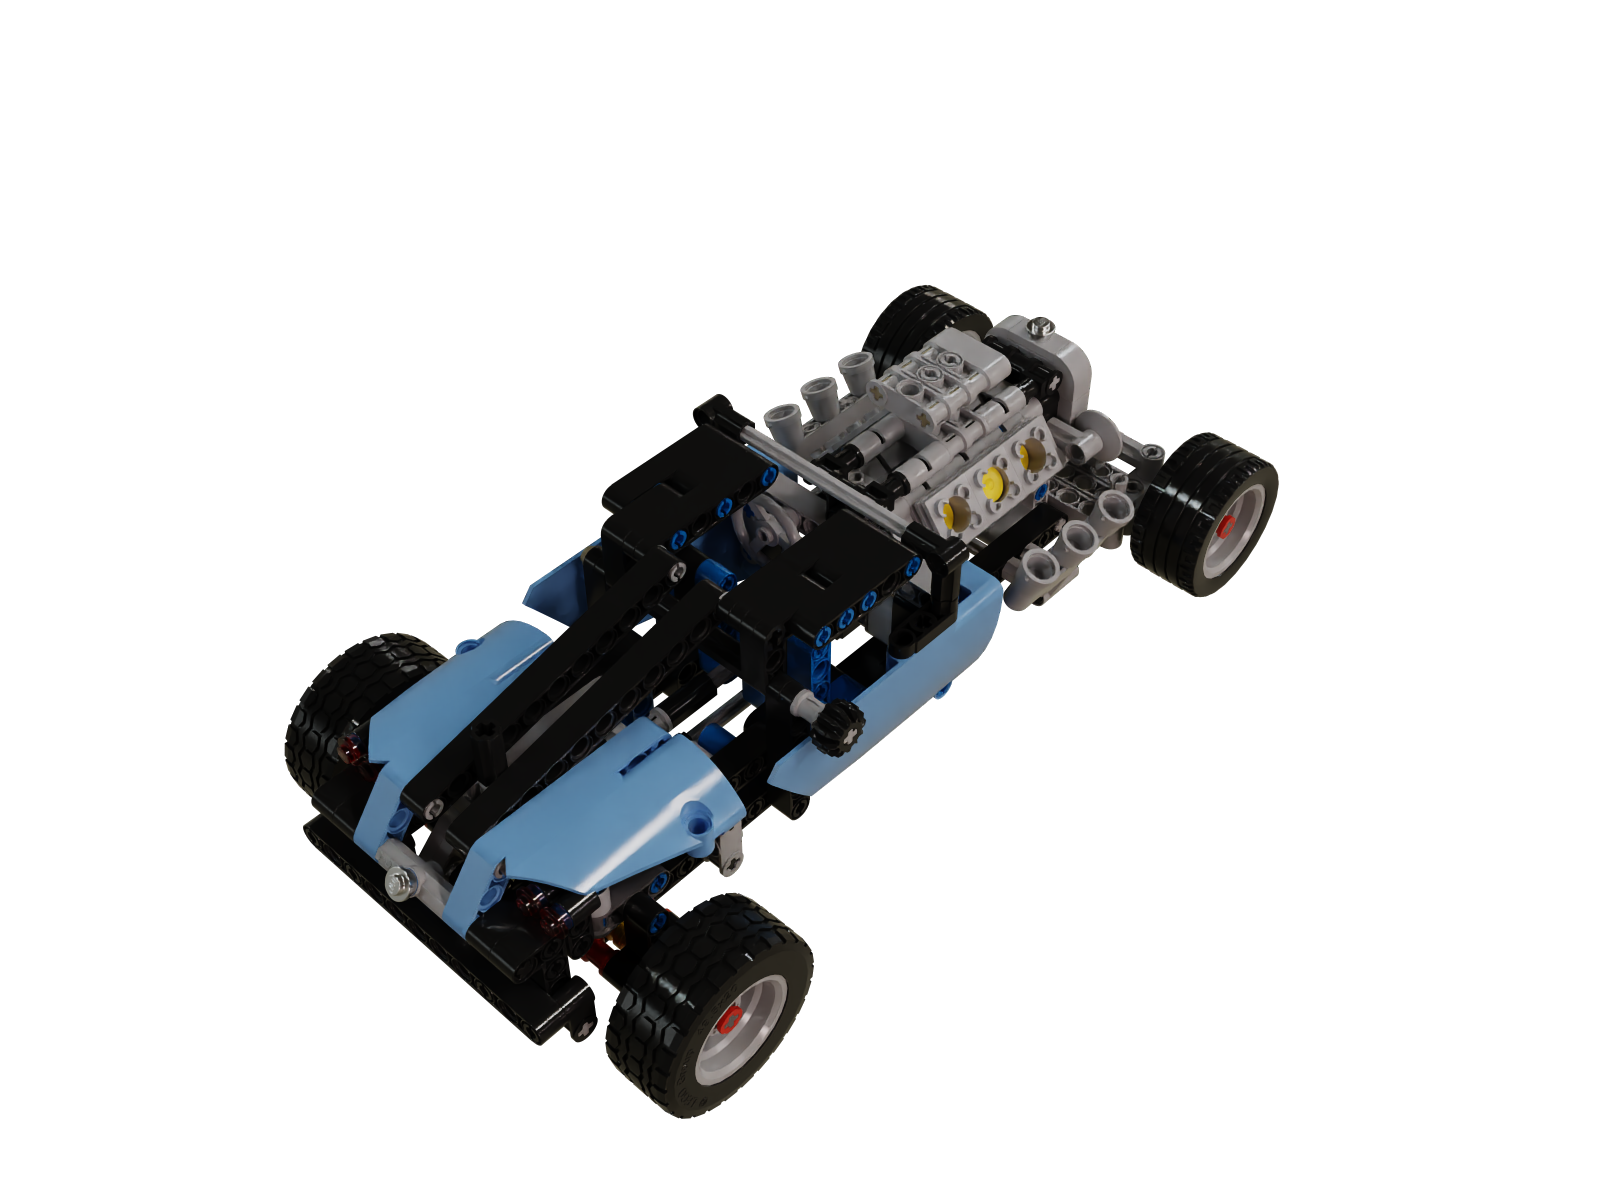
\includegraphics[width=\imagewidth]{Figures/empty_warehouse.png}%
  \label{fig:sp02}%
}

% Row 2
\subfloat[Scéna typu \texttt{lebombo}]{%
  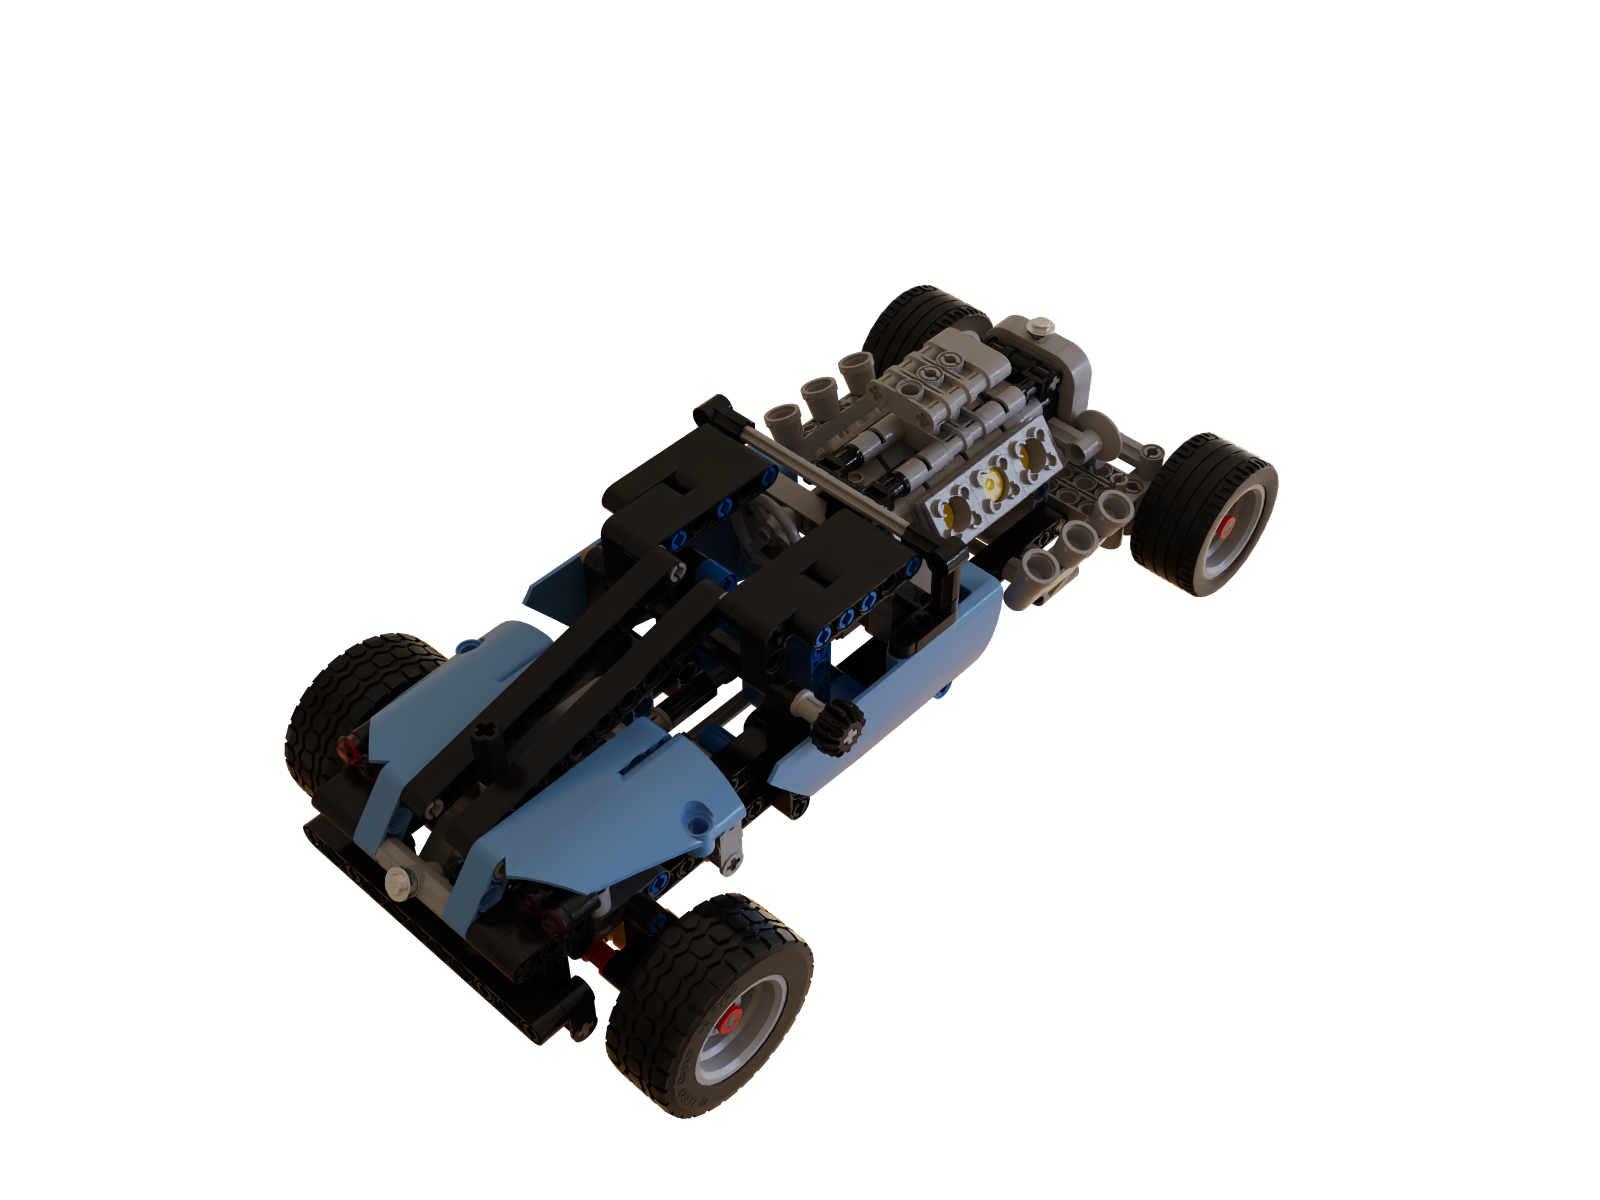
\includegraphics[width=\imagewidth]{Figures/lebombo.png}%
  \label{fig:sp09}%
}\hspace{\hspacesize}%
\subfloat[Scéna typu \texttt{lilienstein}]{%
  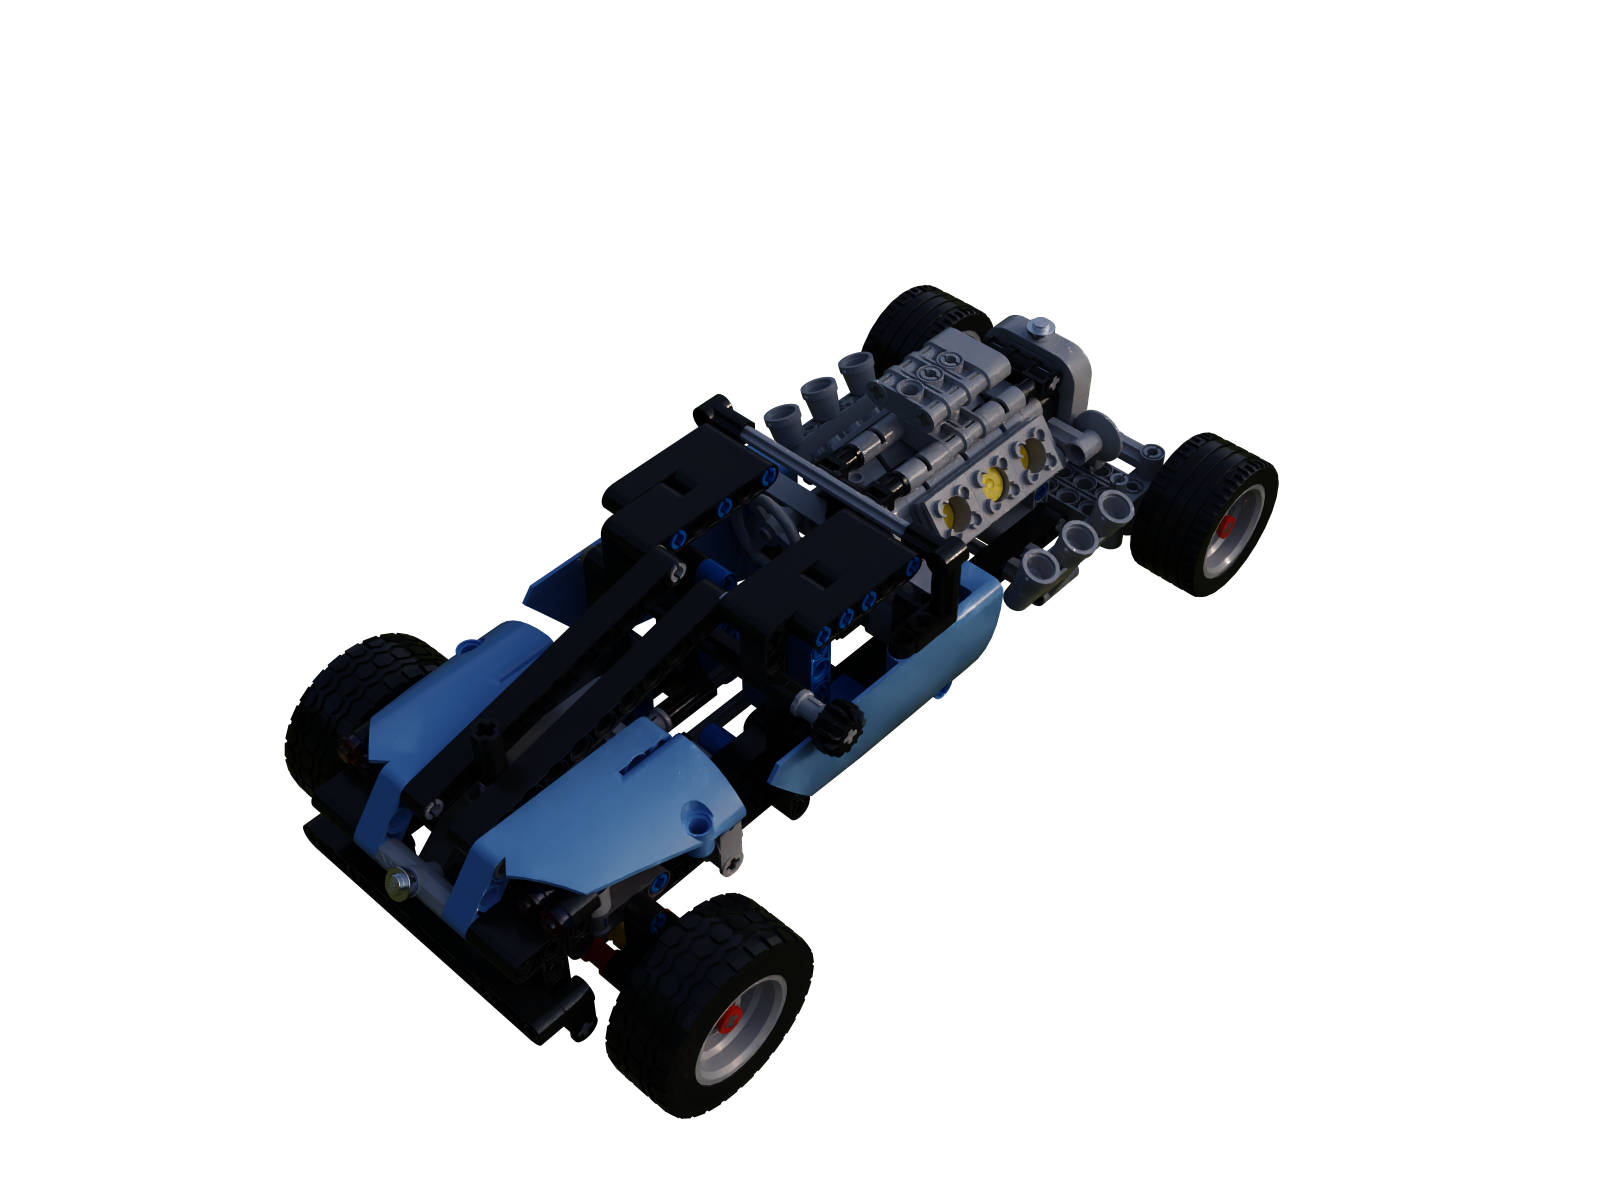
\includegraphics[width=\imagewidth]{Figures/lilienstein.png}%
  \label{fig:sp10}%
}\hspace{\hspacesize}%
\subfloat{%
  \hspace{\imagewidth}
}

\caption[Příklady syntetických snímků z datasetu]{Příklady syntetických snímků z datasetu}
\label{fig:synthetic_images}
\end{figure}


\begin{figure}[hb]
\centering
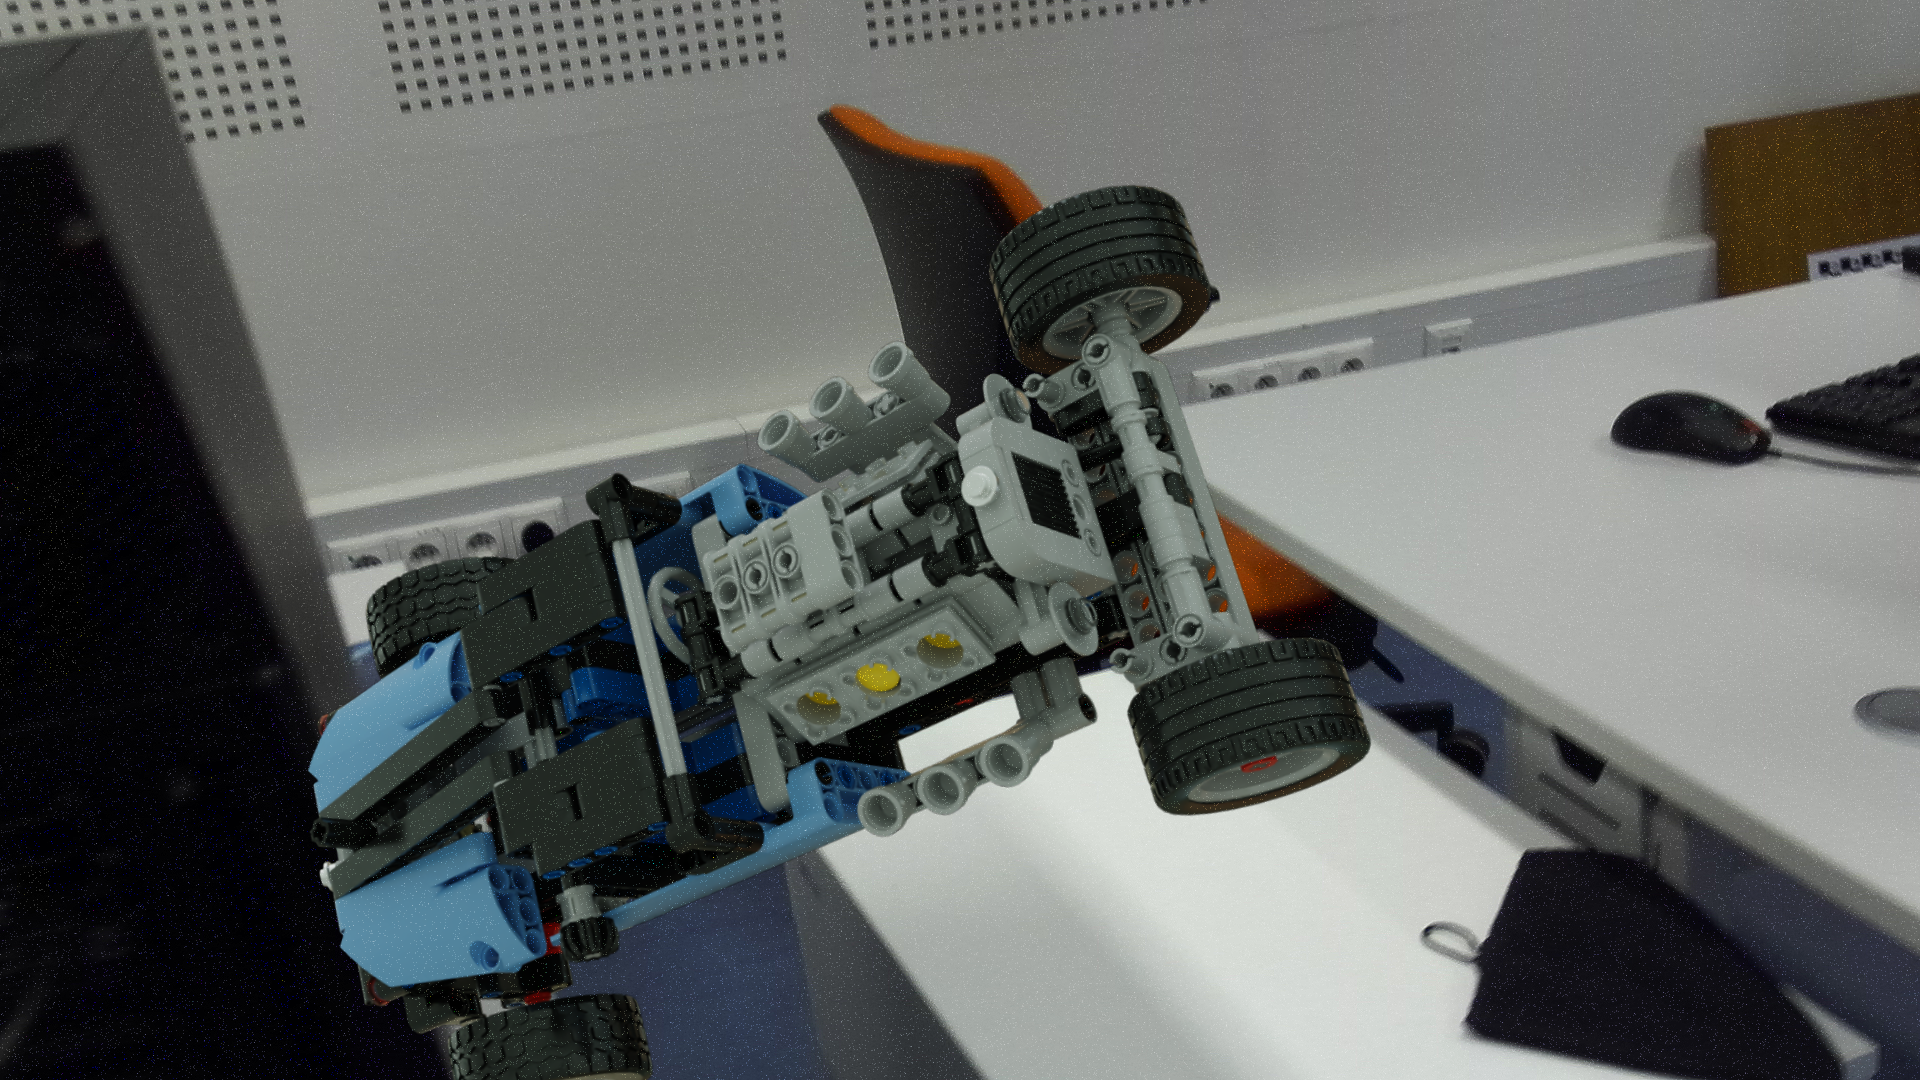
\includegraphics[width=0.4\textwidth,keepaspectratio]{Figures/train_EA408_199.png}
\caption{Příklad kompozitního snímku z datasetu}
\label{fig:trainimg}
\end{figure}
\chapter{Návrh řešení}
\label{sec:Chapter4}
Pro řešení lokalizace klíčových bodů a jejich korespondenci s 3D klíčovými body jsem se rozhodl využít model YOLOv11. Důvodem byla jeho přímá návaznost na populární verzi YOLOv8 a fakt, že YOLOv11 dle oficiální dokumentace nabízí rychlejší a přesnější inferenci, zejména v režimu odhadu pózy na COCO datasetu, což je pro naši úlohu relevantní \cite{ultralytics_yolov8_vs_yolo11}. Klíčové body datasetu jsou definovány bodovými souřadnicemi v kartézském souřadném systému. Ohraničující boxy lze k našim datům snadno vygenerovat, jelikož pozadí je na snímcích vykresleného modelu LEGO auta definováno nulovým alfa kanálem.

% Seznam literatury
\printbibliography[title={Literatura}, heading=bibintoc]

% Prilohy
\appendix
% \input{Chapters/Appendix1.tex}
% \input{Chapters/Appendix2.tex}

% Priloha vlozena primo do hlavniho LaTeX souboru. Ne vsechny prilohy je nutne mit ve zvlastnich souborech.
% \chapter{Dlouhý zdrojový kód}
% \lstinputlisting[label=src:CppExternal,caption={Dlouhý zdrojový kód v jazyce C++ načtený s externího souboru}]{SourceCodes/ArraySortingAlgorithms.cpp}

\end{document}
